\documentclass[11pt]{article}
\usepackage{a4wide}
\usepackage{times}
\usepackage[french]{babel}
\usepackage[T1]{fontenc} 
\usepackage[utf8]{inputenc}
\usepackage{url}
\usepackage{hyperref}
 
\usepackage{eurosym}
\usepackage{amssymb}
\usepackage{xcolor}
\newcommand{\mynote}[3][black]{\textcolor{#1}{\fbox{\bfseries\sffamily\scriptsize{#2}}
{\small$\blacktriangleright$\textsf{\emph{#3}}$\blacktriangleleft$}}}
\newcommand{\pem}[1]{\mynote[cyan]{Pierre-Etienne}{#1}}
\newcommand{\mi}[1]{\mynote[green]{Mireille}{#1}}
\newcommand{\ld}[1]{\mynote[magenta]{Laurence}{#1}}
\newcommand{\TODO}[1]{\mynote[red]{TODO}{#1}}
\newcommand{\TOREMOVE}[1]{\mynote[cyan]{REMOVE}{#1}}
%\newcommand{\TODO}[1]{}
\newcommand{\silent}[1]{}
\newcommand{\gpl}[0]{génie de la programmation et du logiciel\xspace}
\newcommand{\GL}[0]{Génie Logiciel\xspace}
\newcommand{\GDR}{GdR}
\newcommand{\eg}[0]{\emph{e.g.},~}
\newcommand{\ie}[0]{\emph{i.e.},~}
\newcommand{\etal}[0]{\emph{et al.}~}
\newcommand{\wrt}[0]{\emph{w.r.t.}~}
\newcommand{\cf}[0]{cf.~}
%\newcommand{\defi}[1]{\emph{défi~% p.\pageref{#1}, \cite{#1}}}
\newcommand{\defi}[1]{\cite[défi]{#1}}
\newcommand{\defEnum}[1]{\emph{défi~\cite{#1}~p.~\pageref{#1}}}
\usepackage{pdfpages}


\title{{\GDR}~ Génie de la Programmation et du Logiciel\\ 
Défis 2030}
\author{Mireille Blay-Fornarino, Catherine Dubois, Pierre-Etienne Moreau\\
\\
%%\textbf{DRAFT}
}
\begin{document}
\maketitle
\tableofcontents
\section{Introduction}

Le manifeste~\cite{manifeste} rédigé par une partie de la communauté du Groupement de Recherche du CNRS sur le Génie de la Programmation et du Logiciel ({\GDR}~ GPL) commence par ces mots : \emph{Le contraste est saisissant entre, d’un côté, l’omniprésence de l’informatique dans notre
société et la facilité avec laquelle on peut écrire un petit programme, et d’un autre côté, la difficulté extraordinaire de garantir la correction, la fiabilité, les performances ou encore
l’évolutivité d’un logiciel complexe comme on en rencontre aujourd’hui dans tous les pans
de notre société : télécoms, aérospatiale, automobile mais aussi finance, santé,
administration, etc. }
Dans le même temps, l'association nationale néerlandaise pour le génie logiciel publiait également un manifeste ~\cite{Nederland2019} qui reprenait le même argumentaire, mais le complétait à peu près en ces mots:  \emph{Bien que les logiciels aient un impact sur nous tous et partout, l'effort nécessaire pour rendre ces logiciels fiables, maintenables et utilisables sur de plus longues périodes est régulièrement sous-estimé, tant par les développeurs que par leurs responsables. En conséquence, nous voyons tous les jours des articles sur des bogues logiciels coûteux et des projets de développement de logiciels qui dépassent le budget ou qui échouent\footnote{Despite the fact that software impacts everyone everywhere, the effort that is needed to make this software reliable,
maintainable and usable for longer periods is routinely underestimated, both by developers and their managers. As a result,
we see news items every day about expensive software bugs and over-the-budget or failed software development projects~\cite{Nederland2019}.}.}


Le Génie de la Programmation et du Logiciel est au c{\oe}ur de l'activité
informatique. Les concepts, méthodes et outils de conception et de
validation de logiciels constituent les éléments manipulés par les
informaticiens pour maîtriser et automatiser les problèmes qui leur sont 
soumis. Avec l'omniprésence de l'informatique dans notre vie,  que ce soit en termes
d'informatique embarquée, d'intelligence ambiante, d'extension du web au niveau
de la planète, d'intégration dans les objets du quotidien, ou encore avec le
développement de grandes infrastructures de calcul ou de traitement de grandes
masses de données, de nouvelles questions de recherche sont posées.
De nouveaux paradigmes, de nouveaux langages, de nouvelles approches de
modélisation, de vérification, de test et de nouveaux outils dans le domaine
de la programmation et du logiciel devraient voir le jour dans les 5 à 10 ans à
venir, que ce soit pour faciliter la vie des concepteurs de logiciels, pour
modéliser et fiabiliser les logiciels ou encore pour devancer l'évolution
technologique, mais également pour prendre en compte de nouveaux enjeux de
société tels que le développement durable, les économies d'énergie ou la maîtrise des systèmes intégrant de l'intelligence artificielle.

Au sein du {\GDR}~GPL, les équipes de recherche françaises qui travaillent sur ces thématiques ont mis en exergue, en décembre 2019, les défis auxquels elles s'intéressent. Dans cet article, nous en proposons une synthèse, non exhaustive, à destination de lecteurs non nécessairement experts du domaine. Les aspects %recherche 
nécessitant des connaissances expertes sont décrits dans les documents joints ci-après. En 2012 et en 2014, la communauté avait également répondu à un appel à défi; la synthèse des réponses a  publiée dans TSI ~\cite{collet:hal-01345654, duchien:hal-00712942}.


Nous avons choisi d'organiser cette présentation des défis selon trois axes qui sont la fiabilité (\cf\ref{s:fiabilite}), la maintenance (\cf\ref{s:maintenance}) et l'évaluation des logiciels (\cf\ref{s:evaluation}). La fiabilité est un défi majeur pour les logiciels qui sont omniprésents dans nos vies, la maintenance pose des problèmes économiques et écologiques pour notre société, tandis que l'évaluation est au c{\oe}ur même de la méthode scientifique.

\section{Fiabilité des logiciels\label{s:fiabilite}}
La fiabilité d'un logiciel est définie par la norme ISO9126 comme la faculté du logiciel de maintenir un niveau de performance spécifique quand utilisé sous des conditions spécifiques. Elle se décline ainsi en différentes dimensions dont la conformité aux objectifs, la sûreté de fonctionnement, la sécurité, les performances, l'efficacité énergétique\ldots~
C'est un des défis majeurs mis en exergue par nombre de chercheurs dont Xavier Leroy dans son discours inaugural à l'académie des sciences~\cite{leroy:hal-02370113}. Si des avancées majeures ont été obtenues dans les secteurs de la vérification, du test, de la preuve formelle, de la surveillance, il reste de nombreux défis à relever pour rendre les systèmes logiciels plus sûrs et améliorer notre confiance dans ces systèmes. 
Les chercheurs en GPL travaillent à une continuité essentielle entre l'expression d'un problème, la mise en {\oe}uvre et la maintenance de la solution logicielle, continuité qui doit permettre de tracer, vérifier, faire évoluer les applications avec une plus grande fiabilité (cf.~\ref{ss:fiabilite:continuite}). Cette continuité implique de maîtriser non seulement le lien entre la spécification et sa mise en  {\oe}uvre dans différents  programmes, mais également l'exécution du programme, qui dépend des compilateurs utilisés et de l'environnement dans lequel il s'exécute (\cf\ref{ss:fiabilite:execution}). 
L'augmentation des besoins en logiciels et leur omniprésence dans notre quotidien exigent bien évidemment que nous nous assurions de la fiabilité des logiciels produits, mais également que les éléments utilisés pour attester de cette fiabilité soient efficaces au sens où ils permettent de valider de plus en plus de systèmes malgré leur complexité et  que nous puissions en justifier (\cf\ref{ss:fiabilite:confiance}).
Ces recherches relèvent simultanément des champs théoriques et pratiques.


\subsection{De l'idée à la mise en {\oe}uvre\label{ss:fiabilite:continuite}} 
La construction d'un système est aujourd'hui l'affaire de nombreux acteurs, des développeurs aux utilisateurs eux-mêmes, mais également d'exigences multiples voir contradictoires (\eg énergie, sécurité, performance). La composition de ces différentes préoccupations est alors une tâche d'une très grande complexité~\defi{argumentation} qui impose de prendre en compte différents aspects, dont la qualification des services (\eg qualité de service, d'expérience), la sécurité
~\defi{securite} et la mise en place de modèles de coordination~\defi{reconfiguration}.


%\paragraph{Fiabilité par construction}
Depuis plusieurs années, les montées en abstraction portées par l'ingénierie des modèles et des langages ont permis de renforcer la fiabilité des logiciels "par construction" en garantissant le respect des propriétés attendues définies indépendamment des langages et environnements de programmation. 
%Les chercheurs en GPL aspirent ainsi à une continuité entre l'expression d'un problème et les exigences associées, la mise en oeuvre et la maintenance de la solution logicielle.
Néanmoins pour appréhender la fiabilité d'une application dans sa globalité il est nécessaire d'avoir les moyens de décrire avec suffisamment de détails les propriétés spécifiques attendues et de raisonner en intégrant de nombreux paradigmes dont l’exécution du programme par un ou plusieurs processeurs et avec des données ou dans des conditions potentiellement imprévues et ceci dès sa conception \defi{reconfiguration, compilation}. 
%
C'est particulièrement le cas pour les systèmes logiciels qui dépendent d'impératifs du monde réel, tels que les systèmes cyber-physiques. 
On constate des besoins similaires pour les systèmes intégrant de l'apprentissage automatique qui restent difficiles à tester au sens du génie logiciel et pour lesquels les notions de qualités logicielles restent à définir~\defi{IA}.  
De manière générale, la fiabilité des  applications émergentes intégrant  systèmes cyber-physiques et intelligence artificielle, dont par exemple les voitures autonomes, soulèvent  un grand nombre de questions de recherche tant du point de vue de l'expression des propriétés recherchées qui doivent intégrer la modélisation du comportement humain en plus de celui du système ainsi que les liens entre eux, que des outils permettant de les vérifier~\defi{emergents}.

%\paragraph{Sécurité by Design}

\subsection{Du programme à son exécution\label{ss:fiabilite:execution}}
Dans cet objectif de continuité de l'analyse d'un problème à sa mise en {\oe}uvre et maintenance informatique, une étape est tout particulièrement étudiée, celle qui permet de passer du programme à son exécution avec deux  grandes problématiques liées : la preuve et la performance.

Les preuves peuvent s'appliquer à différents niveaux de description d'un programme, de sa spécification à son exécution. 
Cependant la traçabilité entre ces différents niveaux est très difficile à établir. Ceci est d'autant plus complexe que les changements de niveaux induisent à la fois des choix et la prise en compte de nouvelles préoccupations.
Ainsi même si les compilateurs ne sont jamais que des programmes permettant de transformer du code en d'autres programmes, il reste très difficile de les vérifier. En effet, un des intérêts des compilateurs est d'optimiser les exécutions, en s'adaptant aux environnements d'exécution, sans exiger du programmeur de s'intéresser à ces aspects~\defi{Monniaux}.

Si des travaux tels que \textit{CompCert}, un compilateur C optimisant, permettent de garantir mathématiquement la même sémantique entre la source et le programme assembleur généré, la variabilité des environnements d'exécution introduit différents verrous. \\
Ainsi, la variabilité des  plates-formes d'exécution intégrant des processeurs séquentiels, les systèmes distribués constitués d'ordinateurs indépendants dans le nuage ou des ordinateurs quantiques posent  deux problèmes majeurs, la gestion de la cohérence de la mémoire et l'ordonnancement des différentes entités de calcul. Des modèles de programmation et des bibliothèques algorithmiques spécifiques (par exemple MapReduce) ont été définis pour s'adapter à différentes configurations spécifiques, mais ne répondent que partiellement à la problématique de la preuve. La tâche est d'une telle complexité qu'elle nécessite de faire référence à l'expertise en architectures parallèles, en langages de programmation, en calcul haute performance, en typage et en analyse statique, en compilation et en environnements d'exécution \defi{compilation}.

Notons que ces problématiques sous-tendent à la production de logiciels éco-responsables qui utilisent efficacement les ressources en fonction des contextes d'exécution~\defi{vert} et la protection des logiciels d'attaques matérielles~\defi{Monniaux}, tandis que les choix d'architecture impactent non seulement les performances mais également la sécurité des applications produites~\defi{securite}.




\subsection{Des outils pour élaborer la confiance \label{ss:fiabilite:confiance}}
Un des points difficiles dans l'ensemble des éléments relevés précédemment est la construction des éléments de confiance eux-mêmes. Il est indispensable de disposer d'outils qui permettent d'élaborer ces preuves complexes avec plus de facilité, nous retrouvons cette dimension dans \defi{Monniaux, reconfiguration}.  

%\subsection{Informatique de confiance}
Avec quels éléments de preuve est-il raisonnable d'avoir confiance dans un système? Comment justifier qu'un système est bien construit? Ces questions vont au-delà de la preuve ou du test d'un système. Elles nous ramènent à  la problématique de l'accessibilité au raisonnement suivi pour donner confiance dans un système que ce soit ou non dans un objectif de certification \defi{argumentation}.  Elles abordent sous un nouvel angle des verrous tels que la 
complémentarité entre preuves, tests et simulations, les relations entre les artefacts logiciels et les exigences, entre la construction des éléments de preuve et la construction du système, etc. 

\section{Production, maintenance et évolution efficiente des logiciels \label{s:maintenance}}
Les méthodes et techniques introduites par la recherche en génie logiciel modifient les approches classiques du développement du logiciel~\cite{Broy18} qui devient préventif~\cite{Hamilton18}, auto-adaptable~\cite{Chandra2020, murphy19}, plus proche du monde réel avec par exemple la prise en compte de l’utilisateur dans l’écosystème de développement ou la construction de lignes de produits logicielles évolutives~\cite{Marques2019}. Nous avons donc choisi de présenter ici quelques-unes des questions de recherche posées par l'explosion en besoin de production et maintenance des logiciels.


Un grand nombre des systèmes logiciels sont aujourd'hui distribués, concurrents, de très grande taille et appelés à s'adapter automatiquement aux changements de contexte d'exécution (\eg les systèmes Cloud, Fog, Edge et cyber-physiques), ce qui a conduit à accélérer les changements de méthodes et pratiques de production et maintenance des logiciels.   Au-delà d'une question d'agilité, il s'agit de se donner les moyens de produire des logiciels que nous maîtrisons 
et qui s'adaptent à nos besoins (\cf\ref{ss:maintenance:reconfiguration}), sans perdre la dimension éco-responsable sans laquelle le "monde numérique" devient un danger (\cf\ref{ss:maintenance:vert}). 
Pour atteindre ces objectifs, il faut disposer des abstractions adaptées (\cf\ref{ss:maintenance:abstractions}) et prendre en compte l’exigence de maintenance comme une fonctionnalité essentielle des outils de développements~(\cf\ref{ss:maintenance:debugger}). Enfin, l'intelligence artificielle impacte aujourd'hui fortement les approches de maintenance des logiciels, nous introduisons au paragraphe \ref{ss:maintenance:IA} quelques-uns des défis posés.


\subsection{Reconfiguration dynamique et automatique des systèmes \label{ss:maintenance:reconfiguration}}
Comme la structure des systèmes peut être utilisée en cours d'exécution pour découvrir des services ou adapter des composants, une reconfiguration dynamique correcte devient un aspect important de l'exécution du système. La conception d'outils formels intégrés de niveau d'abstraction supérieur pour aider à la conception d'une reconfiguration sûre, tolérante aux pannes et efficace des logiciels distribués est alors essentielle~\defi{reconfiguration}. 
La communauté de recherche aborde  également la question d’auto-optimiser 
l'environnement (objets connectés, maison/industrie du futur)
pour favoriser une transition énergétique et écologique plus large~\defi{vert}.


\subsection{Logiciels durables\label{ss:maintenance:vert}}
Les logiciels qui nous entourent pour être durables doivent répondre aux besoins spécifiques de chacun, y compris dans des contextes métiers particuliers. Le problème est bien connu et les réponses apportées varient des architectures logicielles (en ce moment les micro services) aux langages dédiés, en utilisant différentes techniques dont l'ingénierie des modèles~\defi{coevolution}. 
De manière presque contradictoire 
cette capacité des systèmes à s’adapter conduit parfois à des
\og obésiciels \fg, qui exigent beaucoup de ressources (mémoire, énergie ou temps) par rapport aux tâches qu'ils doivent remplir. Pour pallier ces obésités, 
différentes pistes sont étudiées dont l'exploitation des masses de logiciels pour prédire les consommations, l'utilisation de simulateurs ou l'analyse de dépendances présentées dans le~\defi{vert}.

\subsection{Maintenir, une exigence d'abstraction et de co-évolution\label{ss:maintenance:abstractions}}
L'expression des systèmes et solutions en utilisant les abstractions adaptées en fonction des objectifs est largement exploitée en informatique ~\cite{DBLP:journals/sigcse/Gurer02} pour améliorer l'efficience de la production d'applications que ce soit par exemple dans les formalismes de compositions des exigences, de construction de preuves, de langages dédiés, d'administrations, d'environnement de production de logiciels, etc. Nous nous intéressons ici à leur exploitation tout au long du cycle de vie du logiciel.



Ces dernières années, différents outils ont été élaborés pour permettre aux utilisateurs de définir leurs  propres abstractions afin de construire des langages et environnements dédiés pour augmenter leur productivité. Ces abstractions sont exploitées par composition, génération et/ou configuration de code. La question de la maintenance est alors éminemment complexe puisqu'il s'agit de s'adapter en même temps à l'évolution des concepts, aux mécanismes qui les exploitent, aux cibles, tout en garantissant la \og qualité \fg~des applications construites. On parle alors de co-évolutions. Si le problème est connu, les avancées en \GL~et les données accumulées dans ces processus devraient permettre de proposer des solutions plus automatiques, rapides et efficaces~\defi{coevolution}, et de les prendre en compte dans l'étape difficile de recherche de défauts,  voir le 
~\defi{debuggers}. Une illustration de cette problématique est posée dans le cadre du \defi{combinatoire}, qui pose la question de définir des langages de spécification et de programmation adaptés aux objets de la combinatoire, impliquant la définition de théories logiques adaptées à ces représentations.


La gestion de la co-évolution doit également permettre de minimiser les coûts de maintenance, en particulier lorsque les systèmes sont soumis à des processus de certification. Ainsi, une des pistes étudiées dans le~\defi{argumentation} porte sur l'identification, la traçabilité et la préservation des justifications encore valides après une évolution du système. 



\subsection{Maintenir, une exigence de première classe \label{ss:maintenance:debugger}}
Face à la complexité des logiciels, malgré les grandes évolutions méthodologiques incluant le test et la preuve, il reste difficile aujourd'hui de réparer et adapter les logiciels; quelquefois la simple reproduction d'un comportement est difficile. 
La construction des logiciels et les 
logiciels eux-mêmes utilisent des paradigmes évolués (e.g. concurrences des tâches, présences de modèles  non déterministes dans les architectures, communications par des composants tiers, masses des codes générés). 
La  recherche des défauts ne peut plus être considérée comme une tâche secondaire, elle doit être appréhendée comme une discipline à part entière, à prendre en compte comme un élément essentiel aux développements mêmes des nouveaux supports de production d'application pour une gestion efficace des logiciels~\defi{debuggers}.
Par exemple, comme nous en avons discuté précédemment, les logiciels sont souvent produits par génération de code. Face aux masses de codes ainsi produites, les outils aujourd'hui ne sont pas adaptés qu'il s'agisse de les évaluer~\defi{coevolution} ou de les prendre en compte dans l'étape difficile de recherche de défauts~\defi{debuggers}.


%\subsubsection{La maintenance face aux générateurs de code \label{ss:maintenance:debugger}}
%Comme nous en avons discuté précédemment, les logiciels sont souvent produits par génération de code. La question de la maintenance est alors éminemment complexe impliquant de modifier les générateurs de code qu'il s'agisse d'atteindre de nouvelles cibles ou d'adapter les générateurs aux évolutions des abstractions de plus haut niveaux. Comment appréhender ces co-évolutions ? Comment concevoir les générateurs de codes pour qu'ils supportent celles-ci ? les données existent… 



%\subsection{Maîtriser les logiciels }
%\TODO{Vers plus de fiabilité sur les résultats de recherche en génie Logiciel}

\subsection{\GL~et Intelligence Artificielle\label{ss:maintenance:IA}}
Peut-on parler aujourd'hui de logiciel sans aborder la question de l'intelligence artificielle et du machine learning ?
Le \GL~est historiquement proche de l'intelligence artificielle (IA), en particulier de l'IA symbolique (représentation des connaissances, raisonnements, modèles d'acteurs\ldots). Les chercheurs exploitent depuis des années les travaux dans ce champ d'études et y contribuent largement (\eg lignes de produits logiciels  et extraction de connaissances~\cite{Carbonnel2020}, évolution des systèmes utilisant des ontologies~\cite{Quinton2020}). La relation spécifique à la gestion des masses de données et aux méthodes d'apprentissage statistique a été abordée dans l'ensemble des défis qu'il s'agisse d'utiliser ces techniques ou de servir ce champs de production de logiciels pour, par exemple, assurer la fiabilité des logiciels qui intègrent de tels composants, tester ces systèmes, expliquer\ldots~
Dans~\cite{IA}, les auteurs mettent en exergue différents défis auxquels la communauté du \gpl~s'intéresse actuellement.

\section{Évaluer pour maîtriser la production de logiciels \label{s:evaluation}}
Nous avons choisi de mettre l'accent dans cette dernière partie sur différents travaux qui visent à évaluer la production de logiciels.

%\subsection{Se donner les concepts et outils pour Mesurer}
\paragraph{Évaluer les informations issues du monde réel}
Aujourd'hui des approches formelles permettent de vérifier la sûreté des actions entreprises par un automatisme. Mais lorsque ces actions s'appuient sur les informations issues du monde réel, la précision de ces données et la justesse des informations transmises au système sont alors essentielles. Dans \defi{emergents}, 
des techniques de supervision,
elles-mêmes prouvées correctes, sont donc mises en place pour évaluer la justesse des informations conduisant aux prises de décision dans les véhicules autonomes.
 
 \paragraph{Evaluer les performances des logiciels}
Évaluer et prédire la consommation d'énergie  exige de raisonner à différents niveaux d'abstractions, en intégrant dans le raisonnement les aspects logiciels, réseaux, matériels et nos propres instruments de mesures, de mettre au point de nouvelles techniques de tests et d'analyses de masses de codes, et de prendre en compte la variabilité des usages. Plus largement, à la frontière du \GL,  mesurer la distance entre les gains apportés par le logiciel et sa frugalité en ressources, pour repenser la numérisation dirigée par de nouveaux référentiels est une des pistes de recherches étudiées dans \defi{vert}.


\paragraph{Méthodes statistiques appliquées à la production de logiciels}
La communauté s'intéresse depuis quelques années à évaluer ses propres résultats par des méthodes empiriques~\cite{yu2019characterizing}. Cependant dans le contexte du \GL, les méthodes statistiques classiques ne sont pas toujours adaptées, et d'autres voies devraient être investiguées pour s'adapter au contexte particulier du \GL. En effet, de nombreuses variables influent sur le développement logiciel, dont le domaine d'application, l'équipe, les objectifs. 
Il en résulte la nécessité d'un grand nombre d'expérimentations impliquant beaucoup de développeurs, ce qui, dans un grand nombre d'applications, est impossible en pratique. Il est donc temps de trouver des techniques plus adaptées, notamment en intégrant dans les expérimentations menées les principes de reproductibilité indispensables à la mesure~\defi{GLE} et en travaillant en amont avec l'industrie du logiciel pour produire les données dont nous avons besoin.





\section{Conclusion}
Le \gpl~est au c{\oe}ur du développement logiciel et les défis à relever sont nombreux pour aller vers une révolution numérique  maîtrisée tant au sens de la fiabilité des logiciels produits, de l'efficience dans leur production et maintenance et de notre capacité à comprendre pour faire des choix sensés. Ces différents champs sont abordés par la recherche en \gpl~en France, notamment par des travaux inter-disciplinaires au sein de la science informatique mais également avec d'autres domaines dont les champs applicatifs. 
Ces recherches  portent sur un objet en mouvement, qui connaît des "révolutions" régulières. Elles
exigent une appréhension profonde de la partie théorique des domaines modélisés (\eg mathématiques, biologie, automatisme), la découverte, formalisation, mise en {\oe}uvre et exploitation de nouveaux paradigmes de programmation (\eg  cloud, green computing, introduction de modèles statistiques, informatique quantique) et leur transfert dans les pratiques industrielles qu'il s'agit à la fois d'analyser et d'accompagner. 
Ainsi les apports théoriques et méthodologiques des recherches en \gpl~ s’appliquent aujourd'hui à de nombreuses disciplines scientifiques et techniques.

%% Ce passage reprend quasiment mot pour mot la conclusion de Laurence sur les défis en ..
Dans ce document, nous avons mis en exergue quelques-uns des défis que des
équipes du {\GDR}~GPL souhaitent relever dans les prochaines années. Ce document
n’a pas l’ambition d’être exhaustif, mais il nous semble représentatif de la diversité
des compétences de la communauté française en GPL et de l’intérêt de soutenir ses
recherches.


\addcontentsline{toc}{section}{Remerciements}
\section*{Remerciements}
Nous tenons à remercier l'ensemble des porteurs de défis pour le travail réalisé en cette période si compliquée, sans autre objectif que de partager leurs travaux. Ce travail a été largement soutenu par les membres du comité de programme qui, par leurs retours et discussions, ont {\oe}uvré à une synergie plus intense entre nos différents champs de recherche.
Enfin, les personnes suivantes nous ont plus spécifiquement aidé à affiner ce texte, en apportant leur expertise et leur vision : Alain Giorgetti.

\bibliographystyle{plain}
\bibliography{gdrGPLDefis}
\addcontentsline{toc}{section}{Références}
\addcontentsline{toc}{section}{Défis}

%\subsection{GLE}
\phantomsection
\addcontentsline{toc}{subsection}{\texorpdfstring{\cite{GLE}}{}~:~Vers plus de fiabilité sur les résultats de recherche en génie logiciel}
\label{GLE}
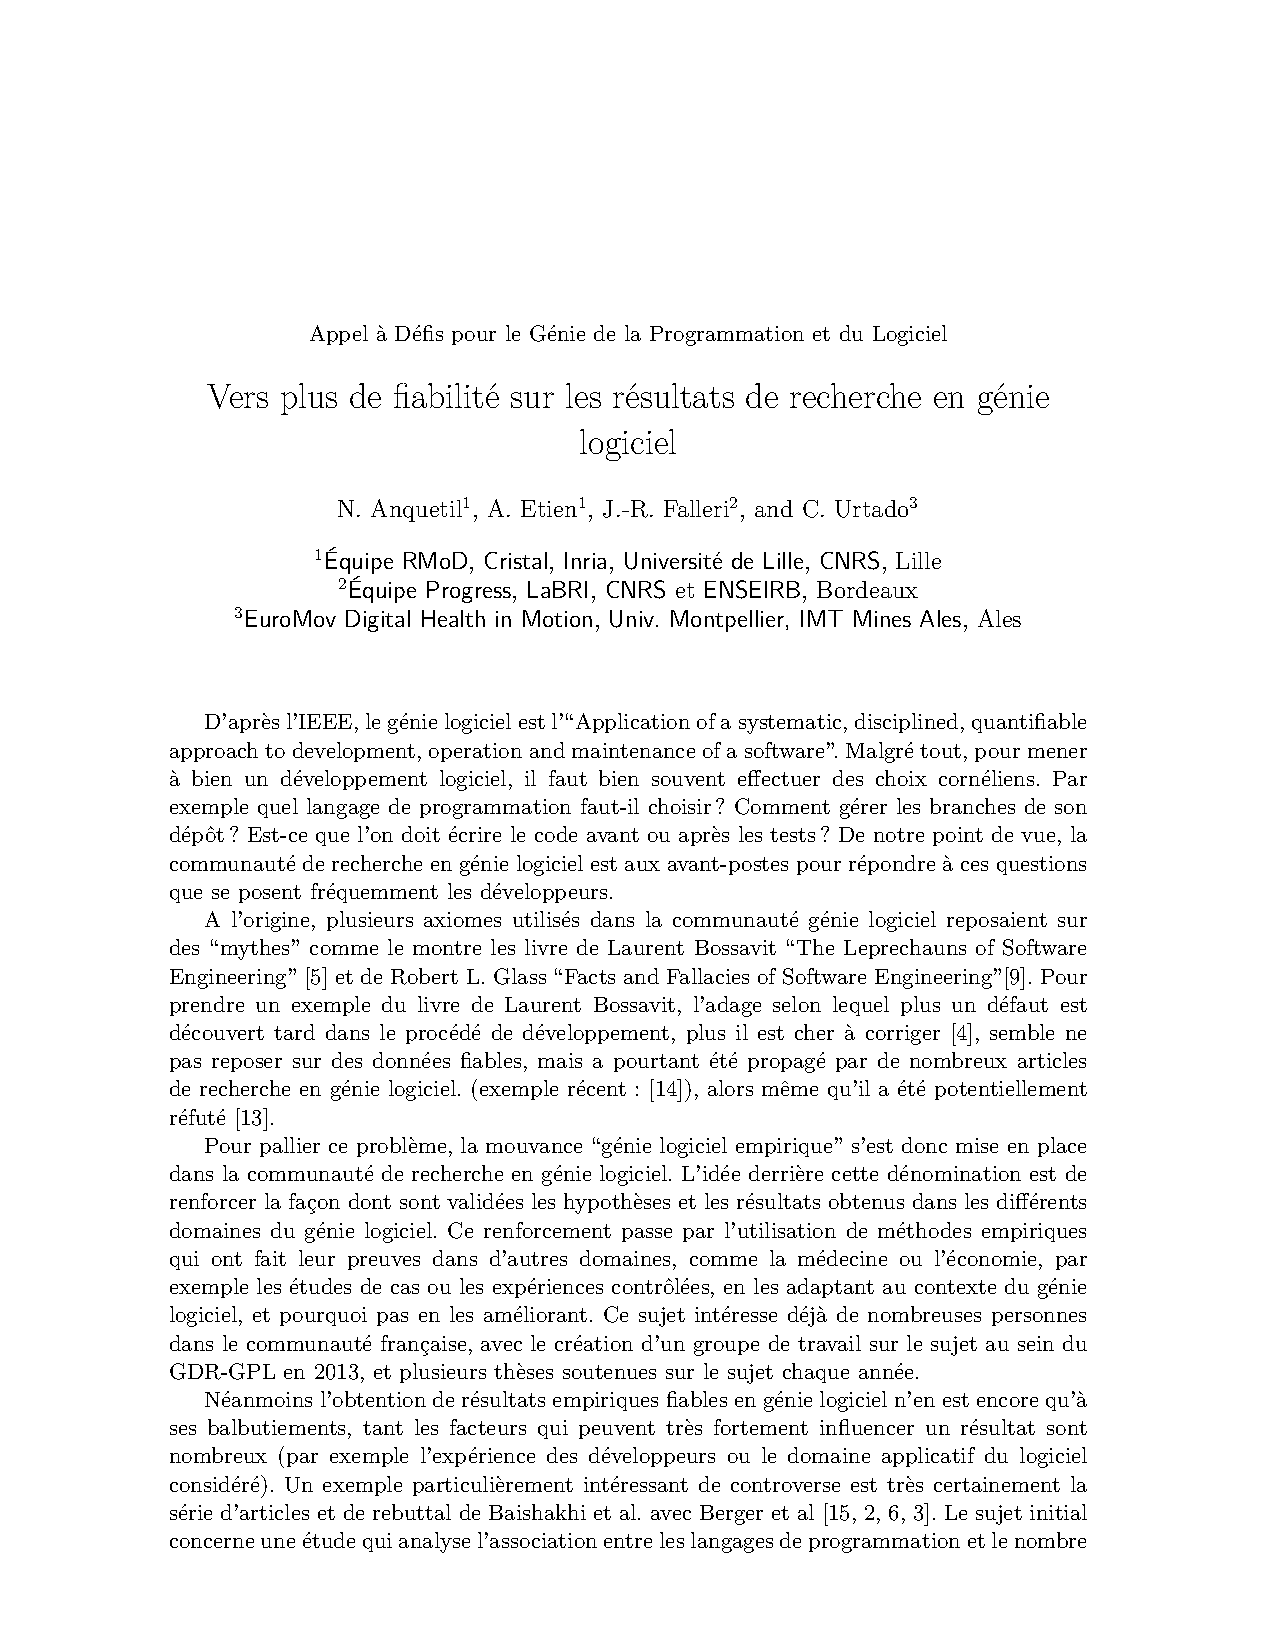
\includepdf[pages=-,pagecommand={\thispagestyle{plain}}]{Defis/Vers_plus_de_fiabilite_Res_recherche.pdf}

%\subsection{reconfiguration}
\addcontentsline{toc}{subsection}{\texorpdfstring{\cite{reconfiguration}}{}~:~Safe and optimal component-based dynamic reconfiguration}
\label{reconfiguration}
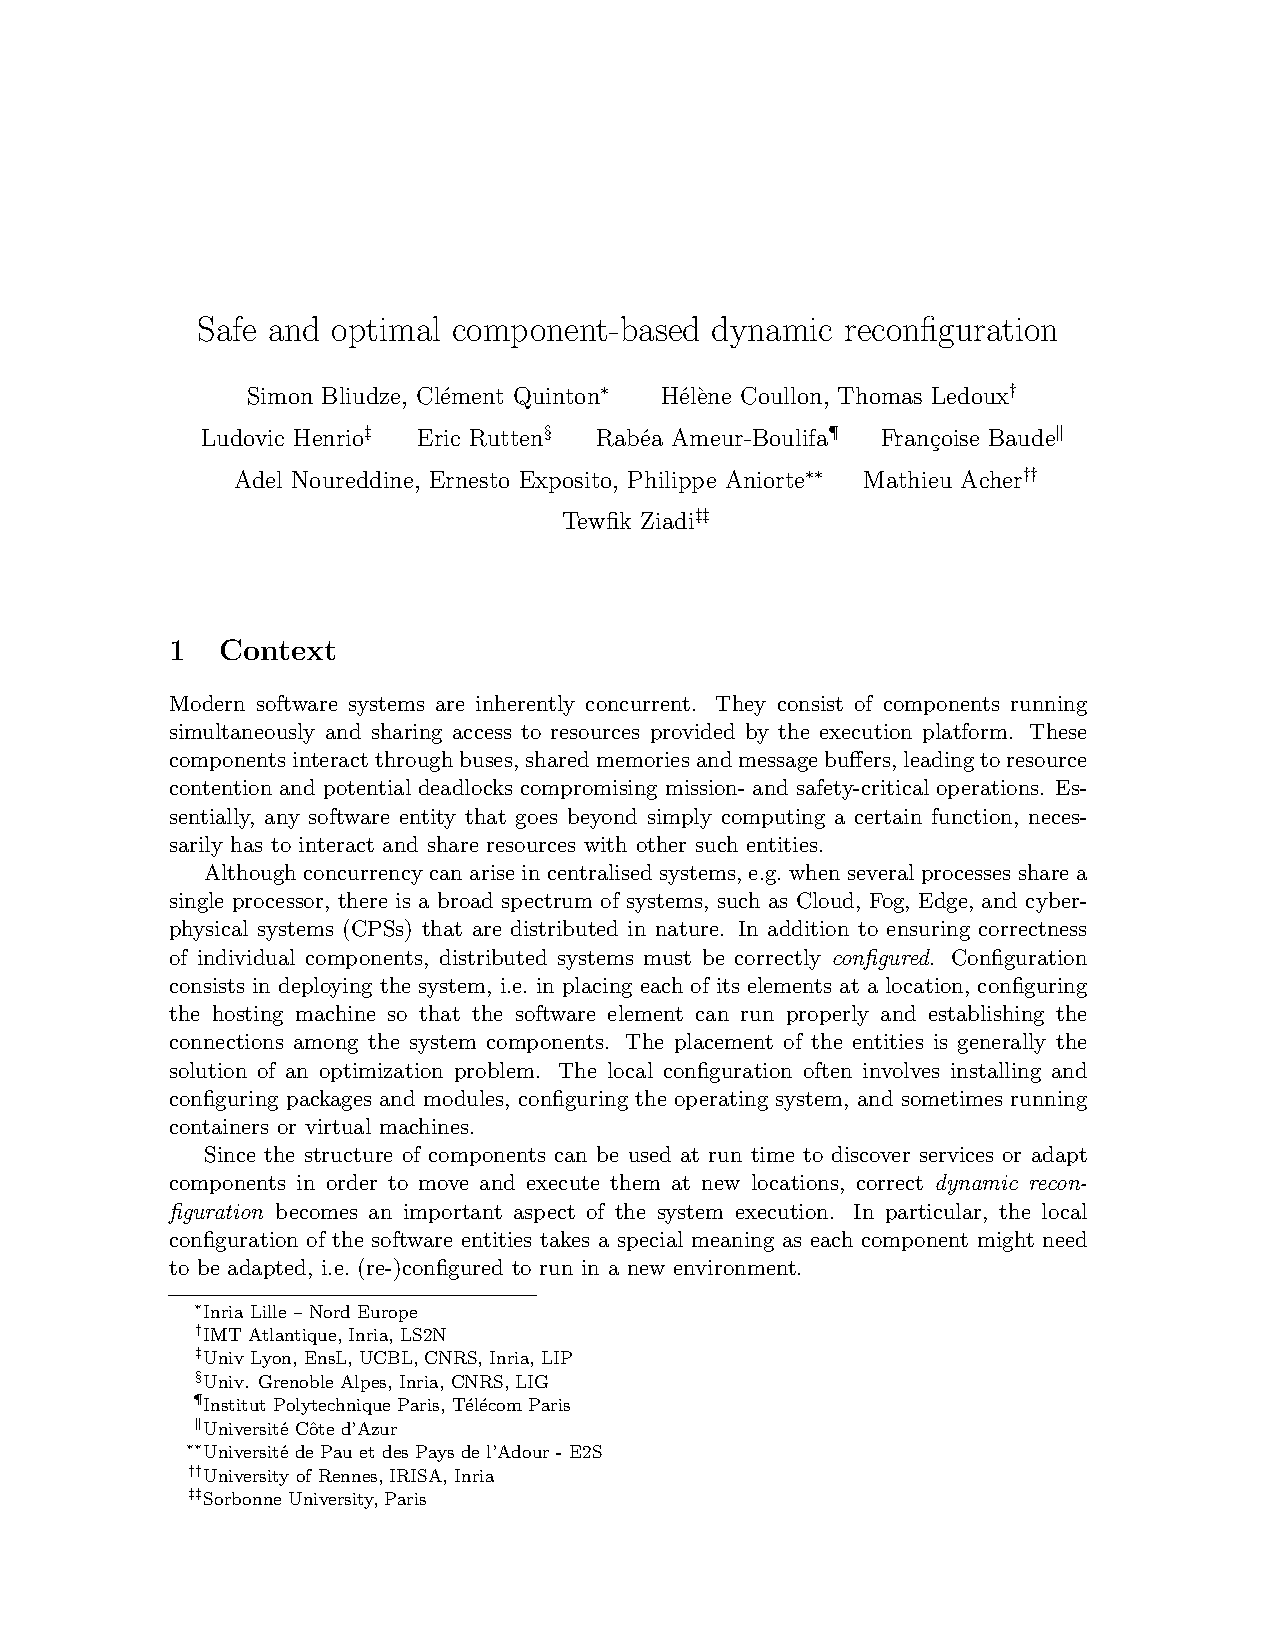
\includepdf[pages=-,pagecommand={\thispagestyle{plain}}]{Defis/Safe_and_optimal_component-based dynamic reconfiguration.pdf}



%\subsection{IA}
\addcontentsline{toc}{subsection}{\texorpdfstring{\cite{IA}}{}~:~Génie Logiciel et Intelligence Artificielle}
\label{IA}
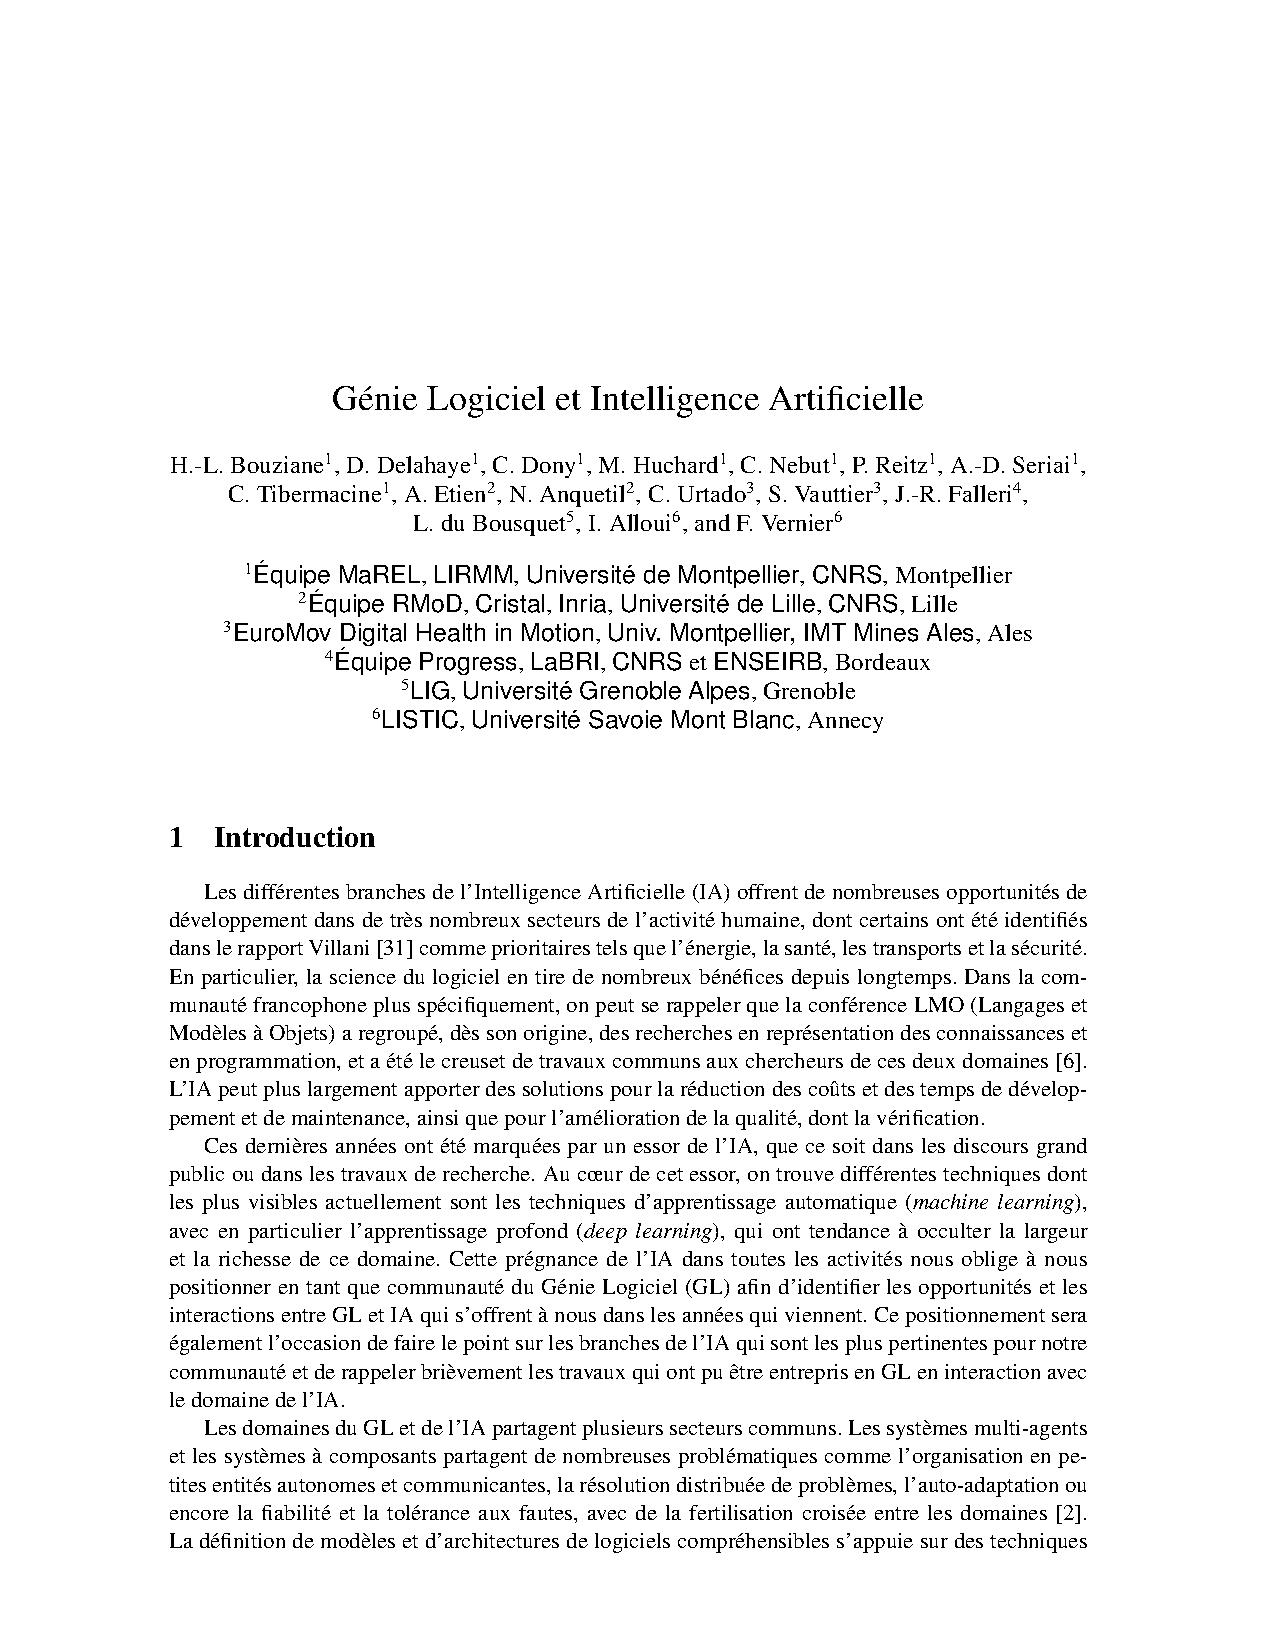
\includepdf[pages=-,pagecommand={\thispagestyle{plain}}]{Defis/Intelligence_Artificielle.pdf}

%\subsection{argumentation}
\addcontentsline{toc}{subsection}{\texorpdfstring{\cite{argumentation}}{}~:~Quelle argumentation pour des systèmes de confiance ?}
\label{argumentation}
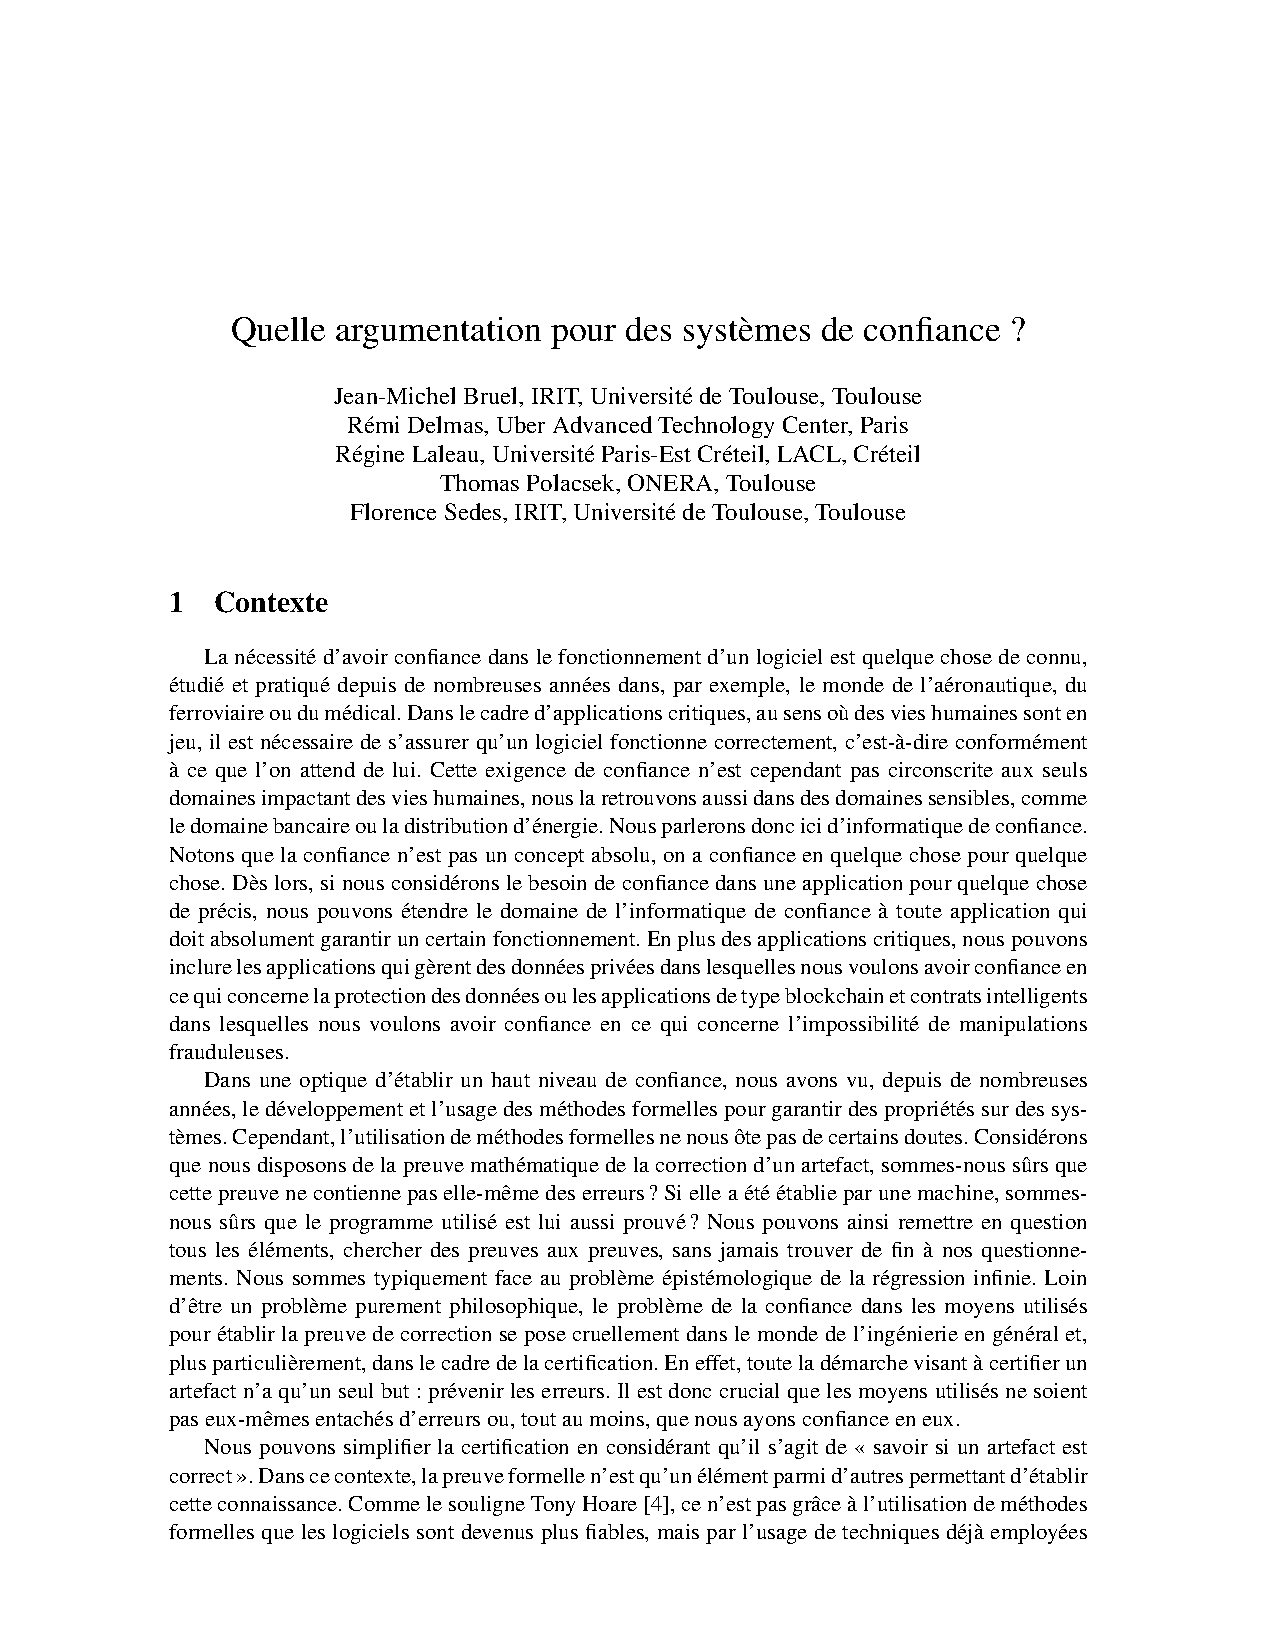
\includepdf[pages=-,pagecommand={\thispagestyle{plain}}]{Defis/argumentation_pour_des_systemes_de_confiance.pdf}



%\subsection{compilation}
\addcontentsline{toc}{subsection}{\texorpdfstring{\cite{compilation}}{}~:~Défi en compilation et langages: du parallélisme oui, mais du parallélisme efficace et sûr!}
\label{compilation}
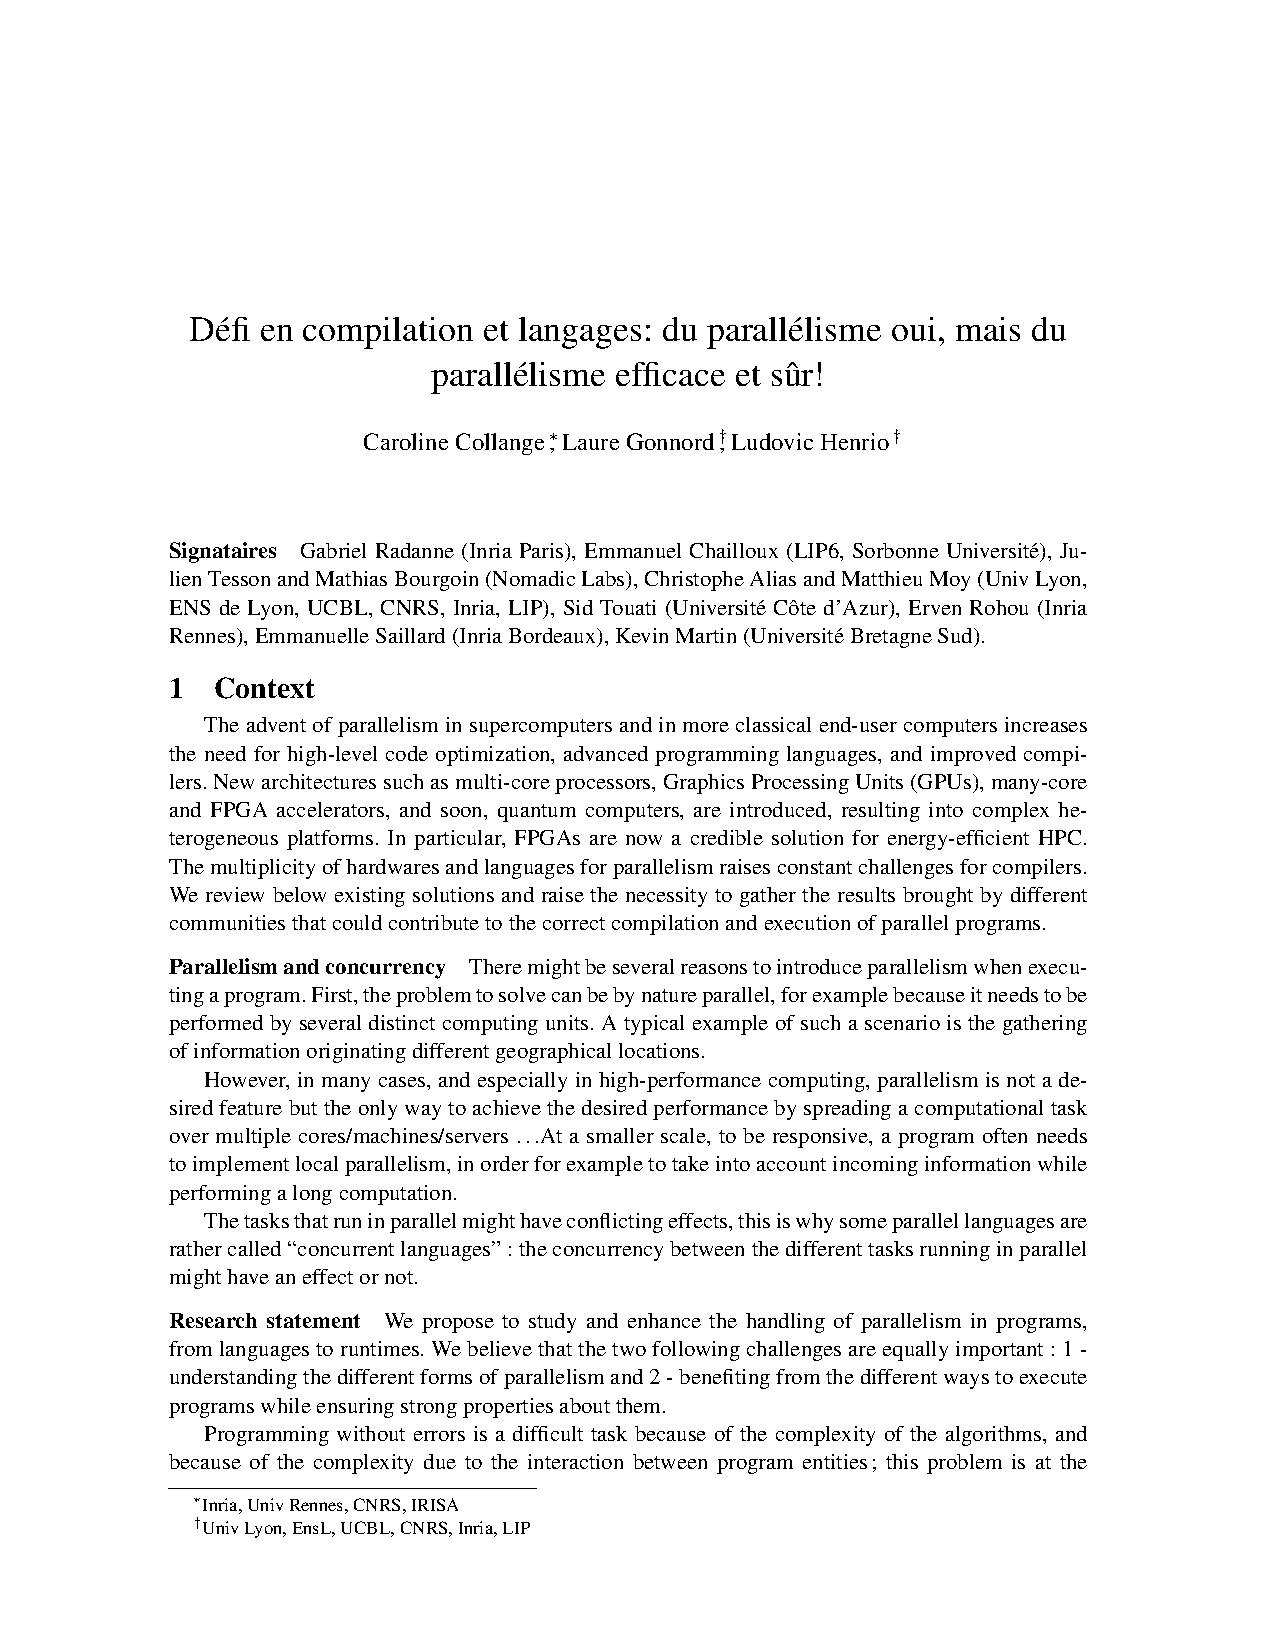
\includepdf[pages=-,pagecommand={\thispagestyle{plain}}]{Defis/Compilation_et_langages.pdf}



%\subsection{emergents}
\addcontentsline{toc}{subsection}{\texorpdfstring{\cite{emergents}}{}~:~Méthodes formelles pour la conception, la programmation et la vérification de systèmes critiques émergents}
\label{emergents}
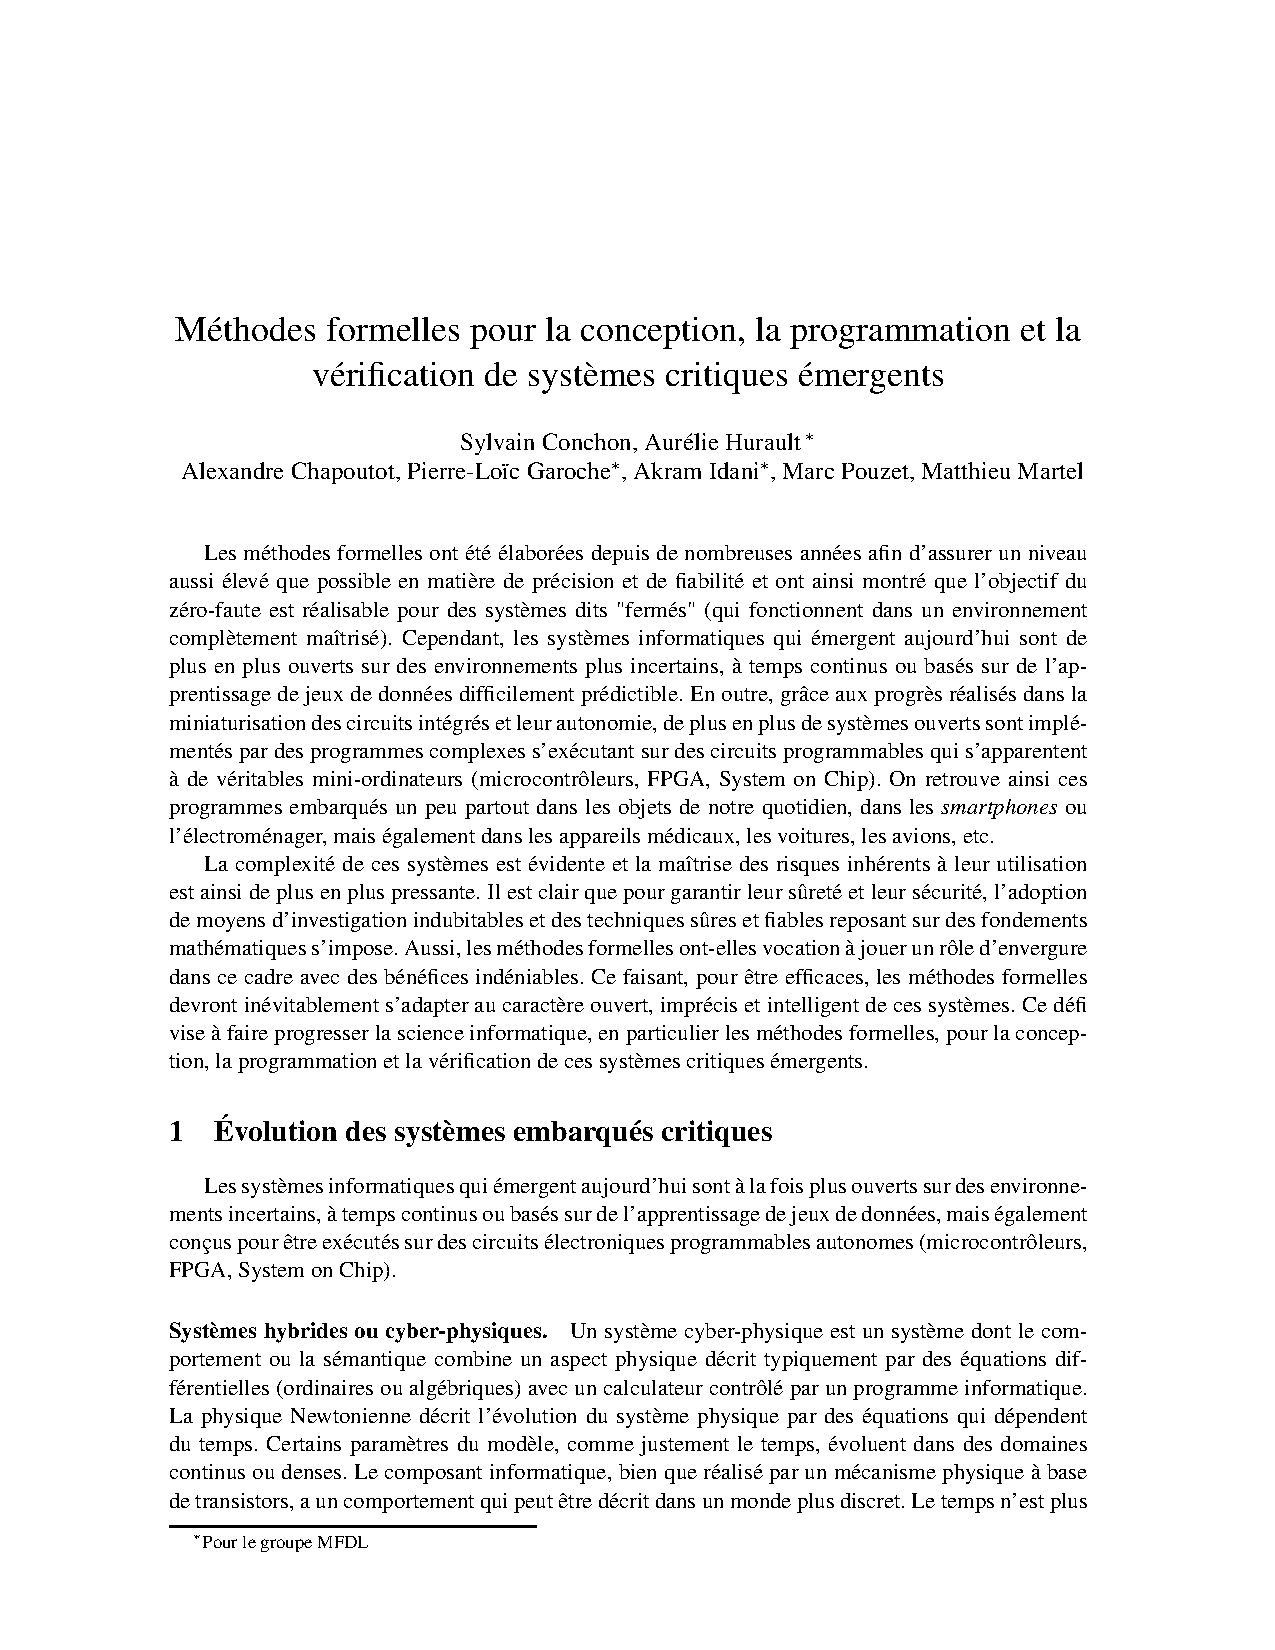
\includepdf[pages=-,pagecommand={\thispagestyle{plain}}]{Defis/FM_systemes_emergents.pdf}

%\subsection{debuggers}
\addcontentsline{toc}{subsection}{\texorpdfstring{\cite{debuggers}}{}~:~New Generation Debuggers}
\label{debuggers}
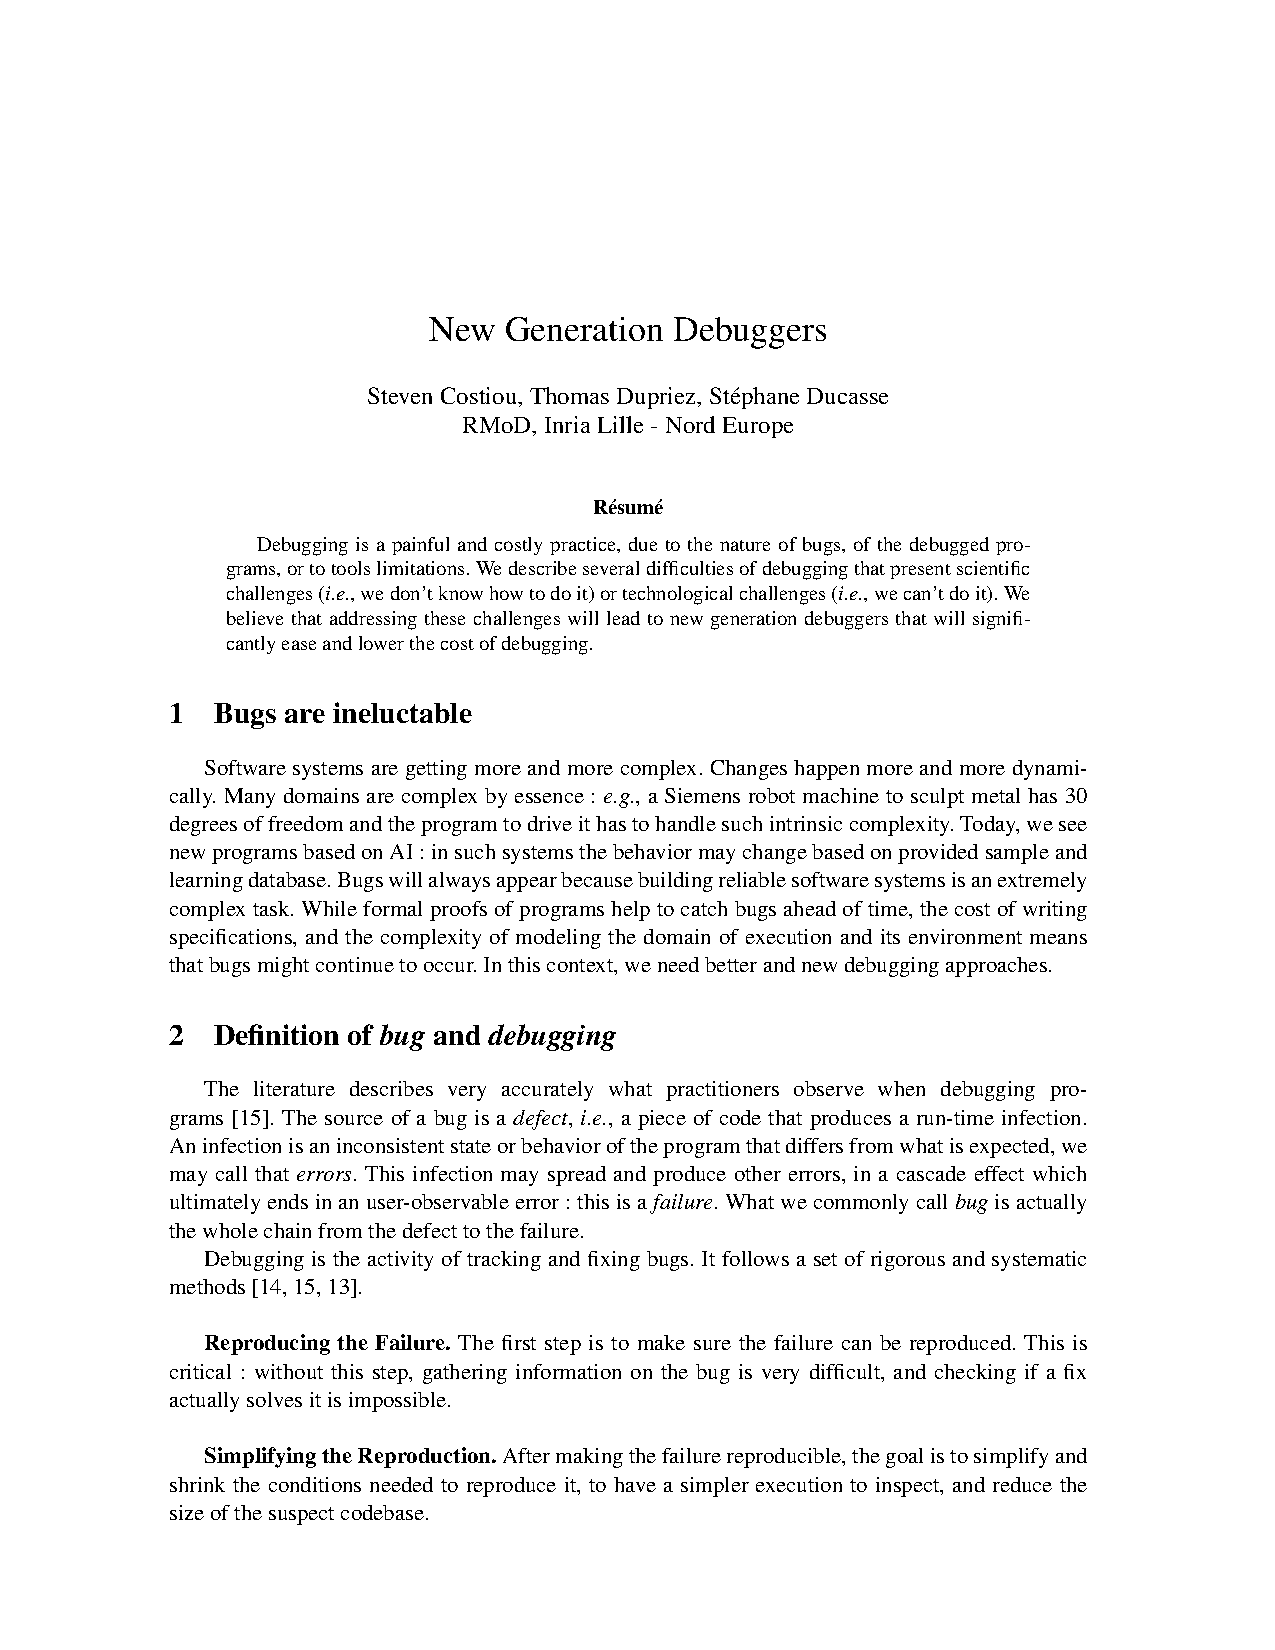
\includepdf[pages=-,pagecommand={\thispagestyle{plain}}]{Defis/New_Generation_Debuggers.pdf}


%\subsection{securite}
\addcontentsline{toc}{subsection}{\texorpdfstring{\cite{securite}}{}~:~La sécurité dans le développement logiciel}
\label{securite}
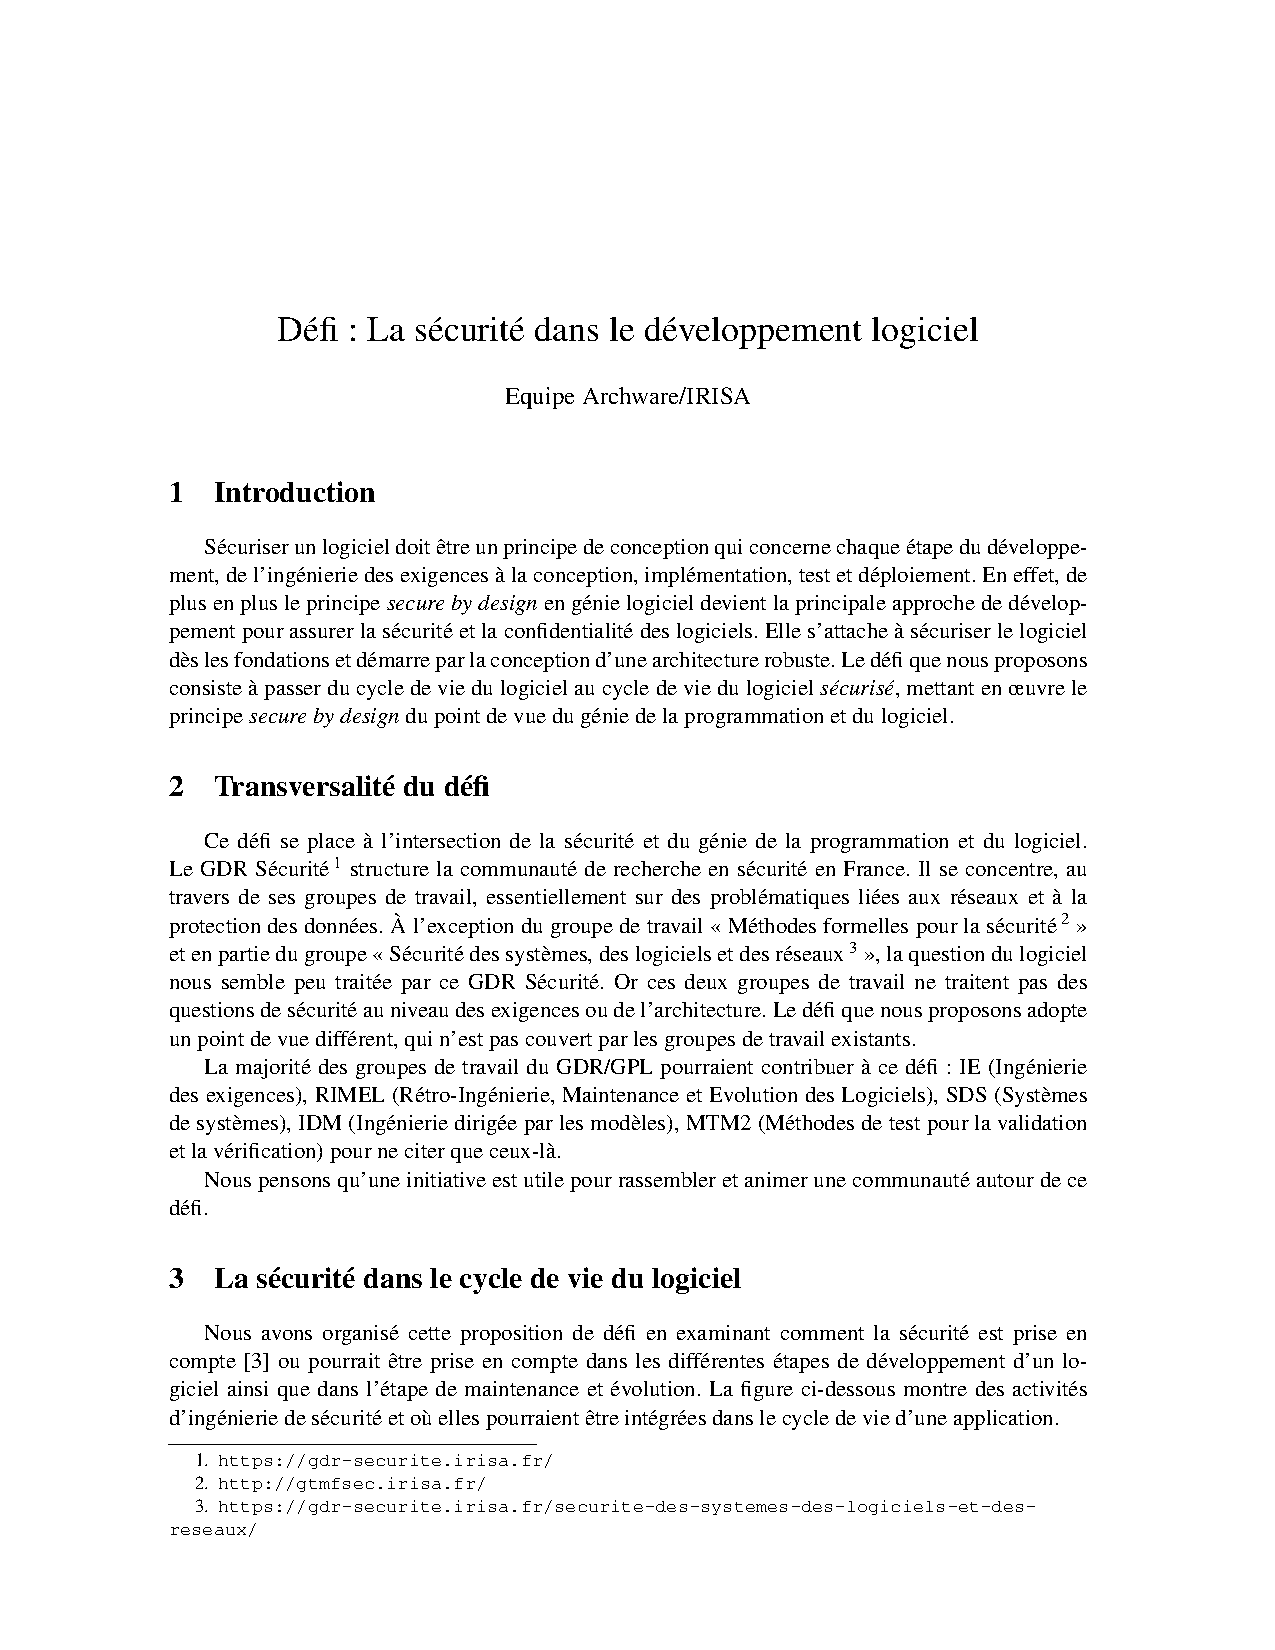
\includepdf[pages=-,pagecommand={\thispagestyle{plain}}]{Defis/securite_dans_le_developpement_logiciel.pdf}

%\subsection{combinatoire}
\addcontentsline{toc}{subsection}{\texorpdfstring{\cite{combinatoire}}{}~:~Combinatoire certifiée}
\label{combinatoire}
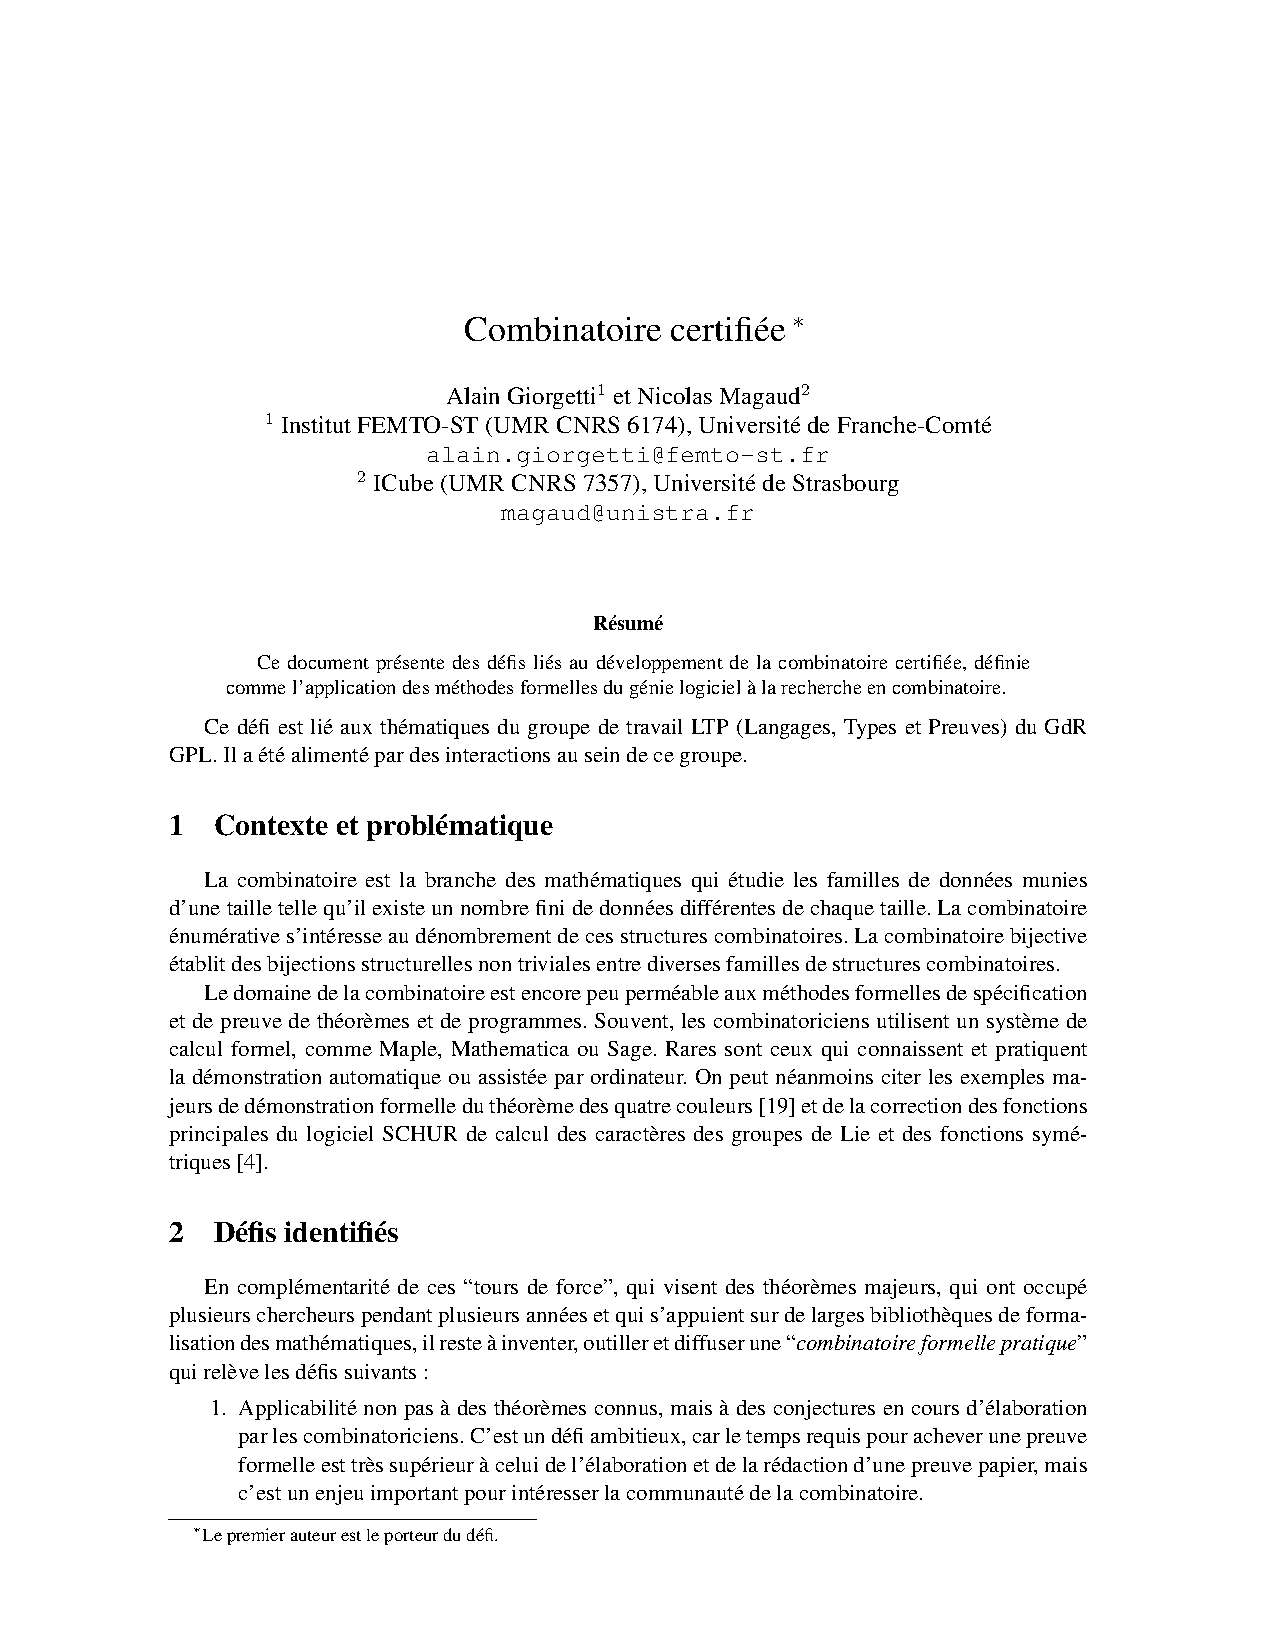
\includepdf[pages=-,pagecommand={\thispagestyle{plain}}]{Defis/combinatoire_certifiee.pdf}


%\subsection{Vert}
\addcontentsline{toc}{subsection}{\texorpdfstring{\cite{vert}}{}~:~Vers des Logiciels éco-responsables, Le génie logiciel au défi de la sobriété écologique}
\label{vert}
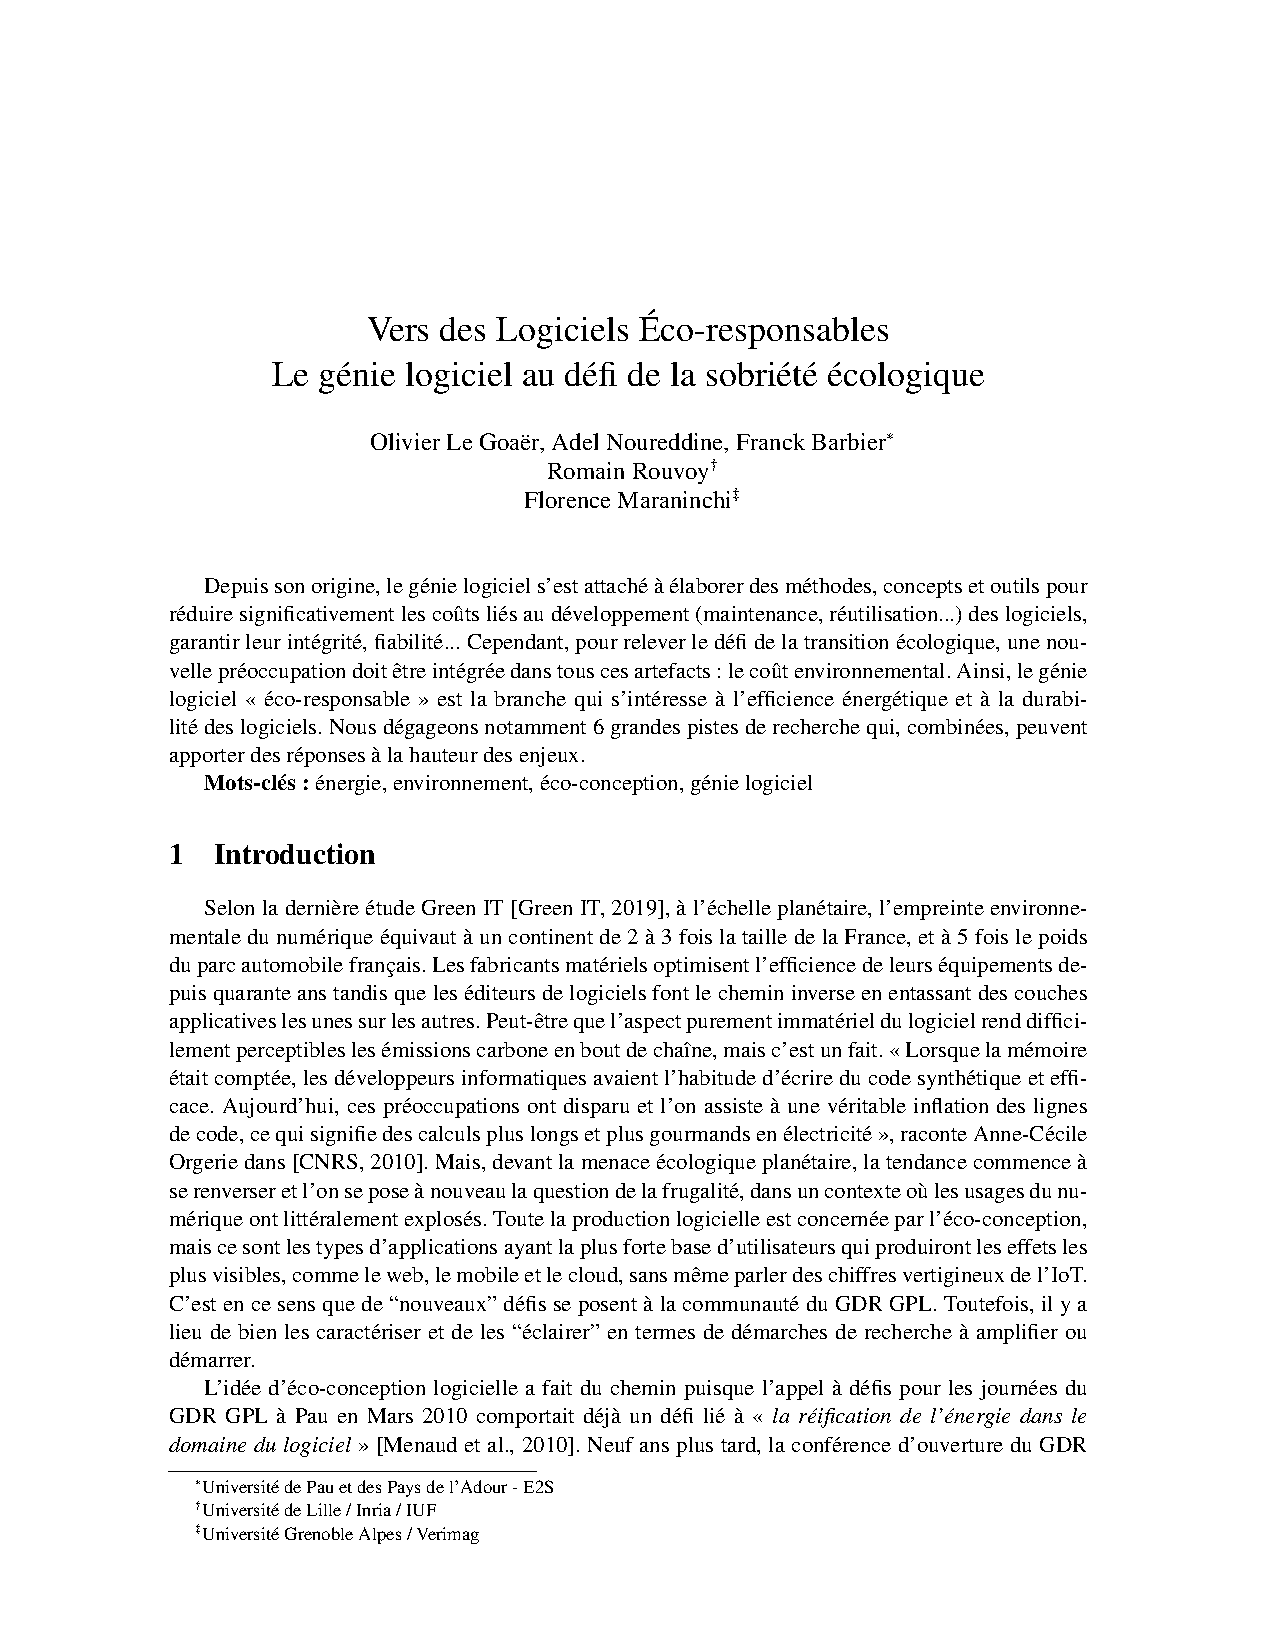
\includepdf[pages=-,pagecommand={\thispagestyle{plain}}]{Defis/logiciels_verts.pdf}

%\subsection{coevolution}
\addcontentsline{toc}{subsection}{\texorpdfstring{\cite{coevolution}}{}~:~Gestion de la co-évolution des logiciels partiellement générés pendant la phase d'évolution et de maintenance}
\label{coevolution}
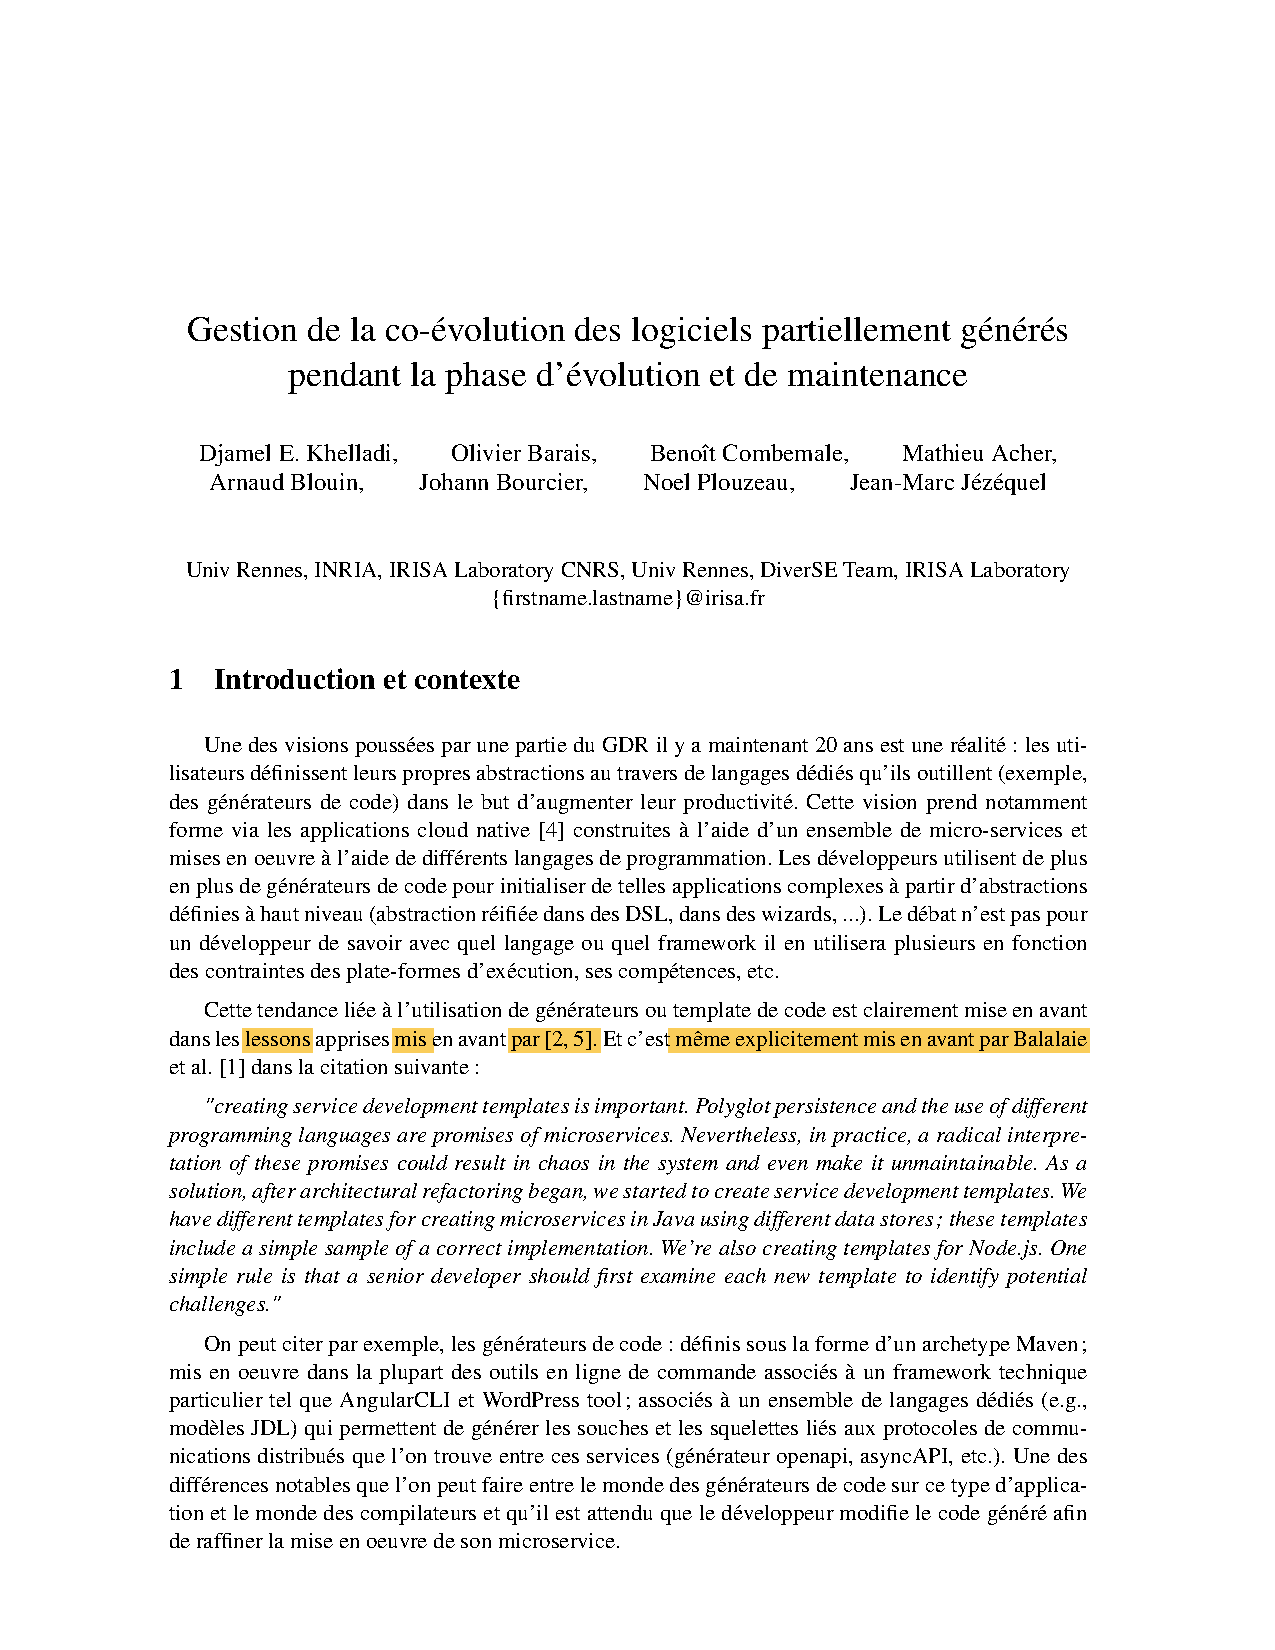
\includepdf[pages=-,pagecommand={\thispagestyle{plain}}]{Defis/co-evolution_des_logiciels.pdf}



%\subsection{Monniaux}
\addcontentsline{toc}{subsection}{\texorpdfstring{\cite{Monniaux}}{}~:~Chaîne de compilation formellement certifiée.}
\label{Monniaux}
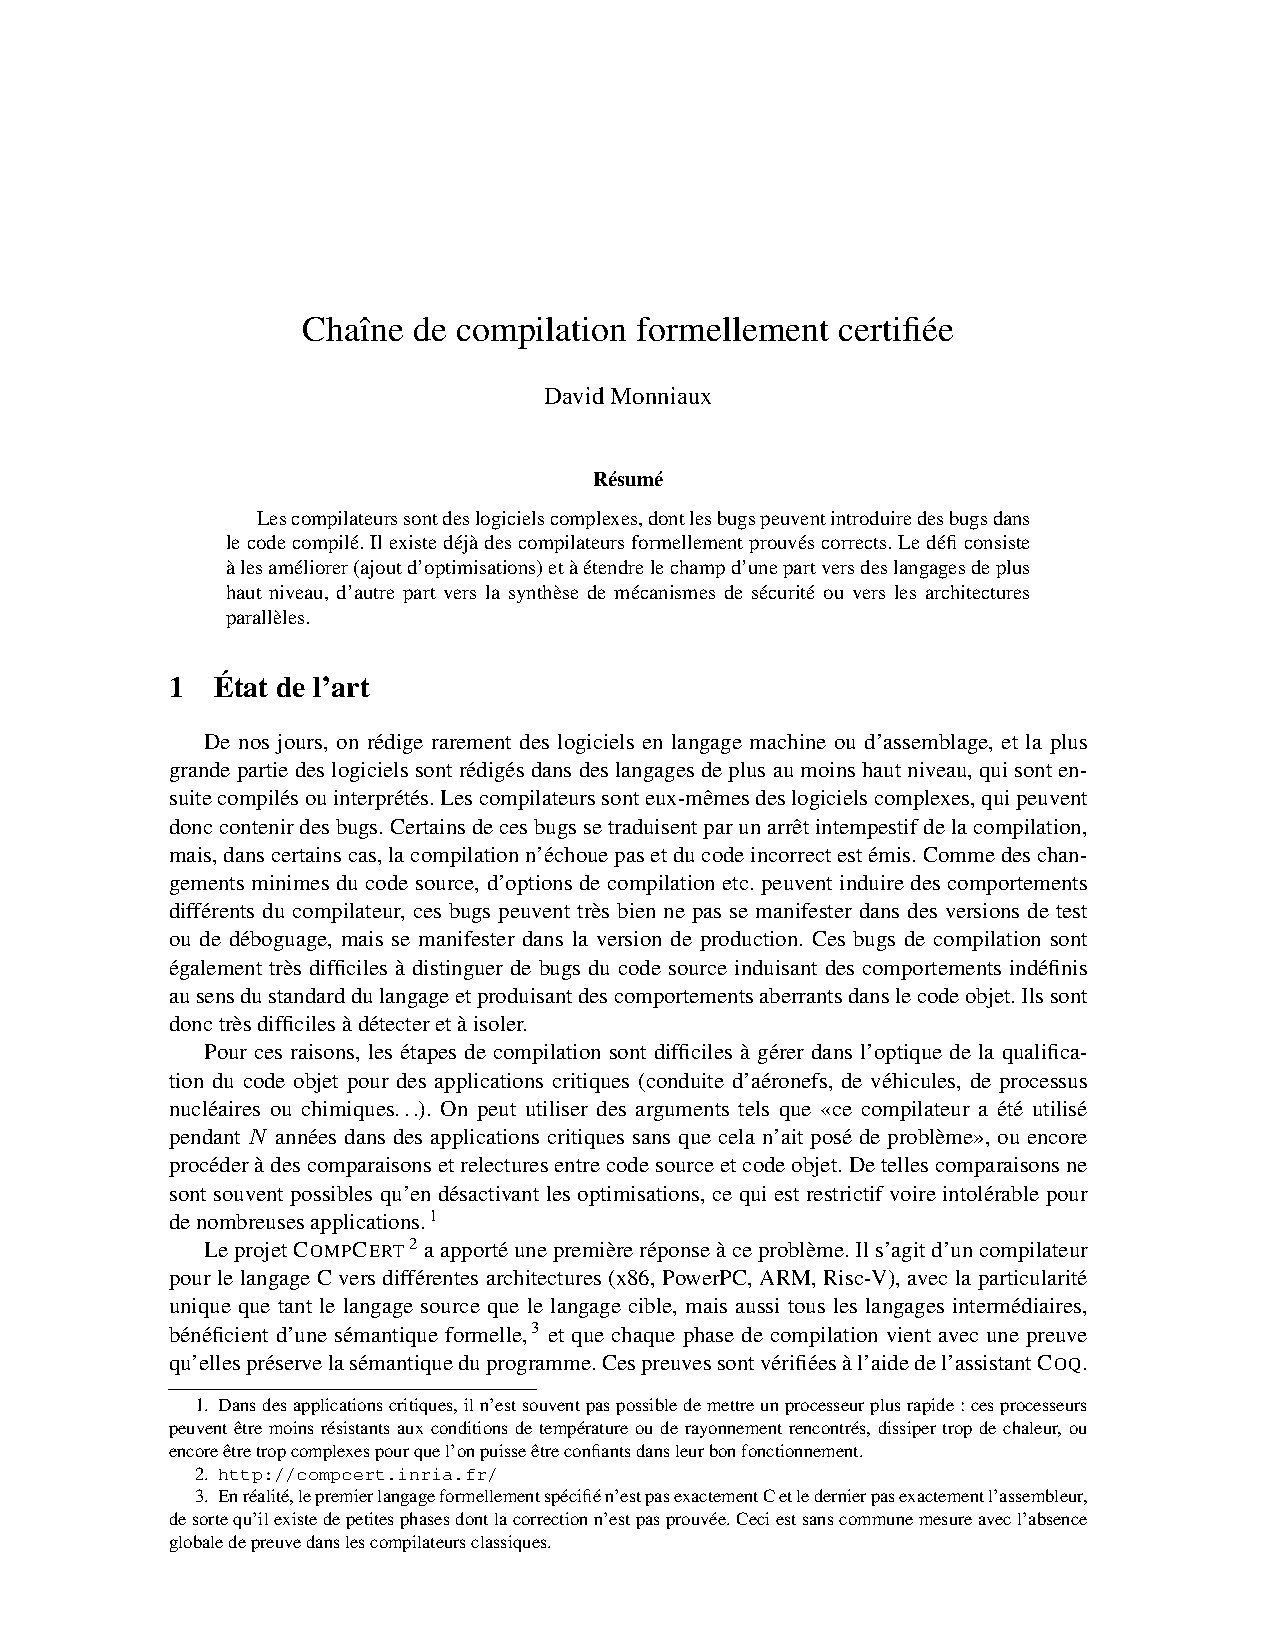
\includepdf[pages=-,pagecommand={\thispagestyle{plain}}]{Defis/chaine_compilation_certifiee.pdf}


\end{document}
